% !TEX root = main.tex
\chapter{Das \lhcb-Experiment}

Das $\lhcb$-Experiment ist neben $\atlas$, $\cms$ und $\alice$ eines der vier großen Experimente am europäischen Kernforschungszentrum $\cern$. Das Experiment ist auf Präzisionsmessungen der Physik von Prozessen mit $\bquark$- und $\cquark$-Quarks spezialisiert. Im Folgenden wird zunächst kurz auf den Large-Hadron-Collider ($\lhc$) eingegangen, um danach den $\lhcb$-Detektor und seine Komponenten detaillierter zu beschreiben (basierend auf \cite{Alves:2008zz}). Am Ende des Kapitels folgt ein Abschnitt über das LHCb Software Framework.

\section{Der $\lhc$}

\begin{figure}[htpb]
	\centering
		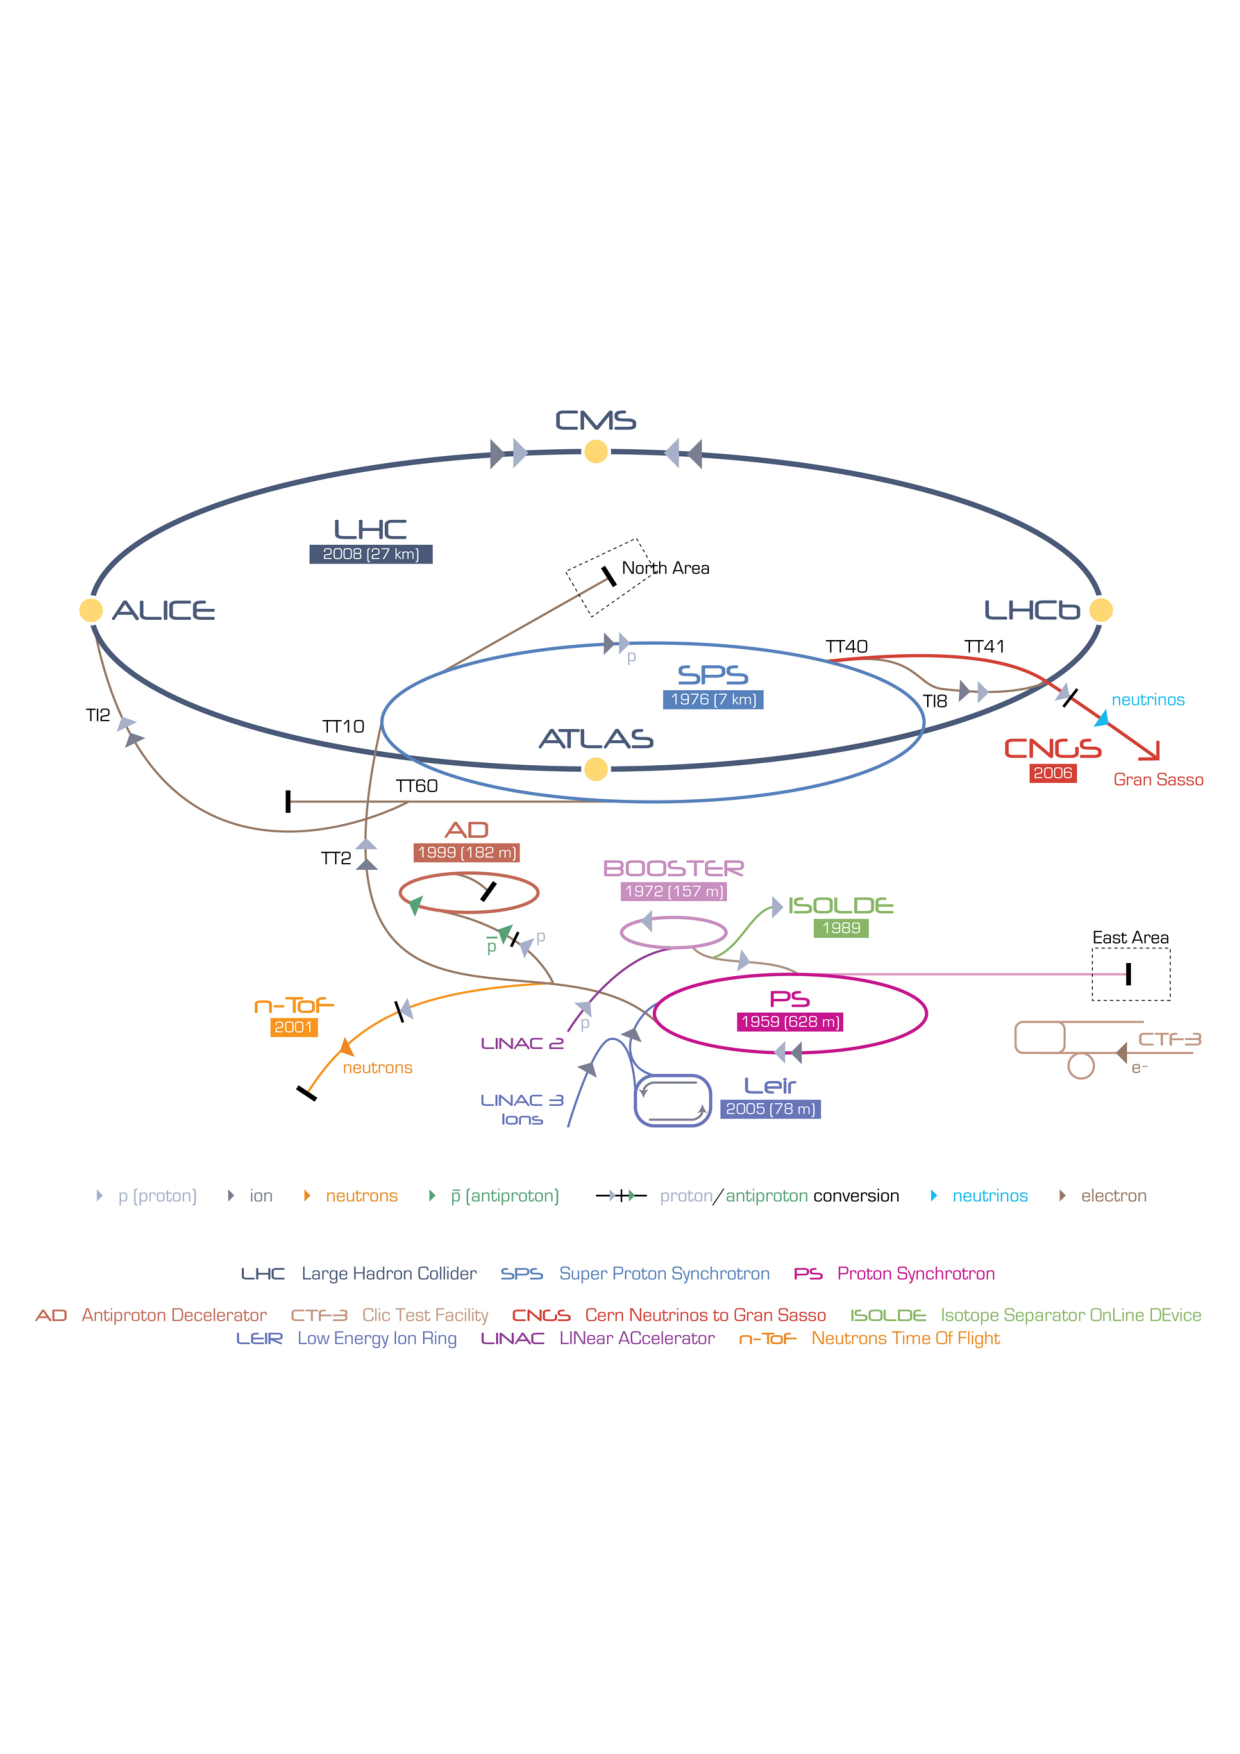
\includegraphics[width=0.75\textwidth]{fig/cern_scheme.pdf}
	\caption{Schematische Darstellung des $\cern$-Beschleuniger Komplexes. Die Protonen für den $\lhc$ werden zunächst im LINAC 2, im Booster, im Proton Synchrotron ($P\!S$) und im Super Proton Synchrotron ($S\!P\!S$) auf eine Energie von \SI{450}{GeV} vorbeschleunigt. Ihr Weg ist in der Abbildung durch die hellgrauen Pfeile gekennzeichnet \cite{cern_scheme}.}
	\label{fig:cern_scheme} 
\end{figure} 
Der $\lhc$ ist ein Ringbeschleuniger am $\cern$ bei Genf mit etwa \SI{27}{km} Umfang. Er ist dafür konstruiert, Protonen bei einer Schwerpunktsenergie von bis zu $\sqrt{s}=\SI{14}{TeV}$ bei einer Luminosität von \SI{e34}{cm^{-2}s^{-1}} \cite{lhc_design} kollidieren zu lassen. Dazu kreisen zwei entgegengesetzte Protonenstrahlen (Beams) im Beschleunigerring und werden an vier Punkten zur Kollision gebracht. \\
Bei den in dieser Arbeit verwendeten Daten bestanden die Beams aus etwa \num{1380} Protonen-Paketen, die jeweils \num{1{,}15e11} Protonen enthalten \cite{LHC_statistik}. Die Anzahl Pro\-tonen-Pakete pro Beam wird voraussichtlich nach dem Long-Shutdown $1$ ($L\!S1$) auf $2808$ \cite{lhc_design} gesteigert. \\
Bevor die Protonen in den $\lhc$-Beschleunigerring eingespeist werden, müssen sie vorbeschleunigt werden. Dies geschieht zunächst in einem Linearbeschleuniger, dem LINAC 2. Darauf folgen der Booster, das Proton-Synchrotron ($P\!S$) und das Super-Proton-Synchrotron ($S\!P\!S$) die allesamt Ringbeschleuniger sind. Aus dem $S\!P\!S$ werden die Protonen dann schließlich mit einer Energie von \SI{450}{GeV} \cite{lhc_design} in den $\lhc$-Ring eingespeist (Abbildung \ref{fig:cern_scheme}). Um die nahezu lichtschnellen Protonen auf ihrer kreisförmigen Bahn zu halten, sind  \num{1232}  supraleitende Dipolmagnete mit einer Länge von jeweils \SI{14{,}3}{m} und einer Feldstärke von bis zu \SI{8{,}33}{T} nötig. Die ersten Protonen im \lhc wurden im Jahr \num{2008} beschleunigt.\\
Insgesamt sind, wie bereits erwähnt, vier große Experimente am $\lhc$ in Betrieb. Bei $\atlas$ und $\cms$ handelt es sich dabei um Mehrzweckexperimente, die bei maximaler Luminosität experimentieren, $\alice$ untersucht vor allem Quark-Gluon-Plasmen. Das vierte Experiment, $\lhcb$, beschäftigt sich primär mit Präzisionsmessungen im Bereich der Flavour-Physik, vornehmlich mit $\bquark$- und $\cquark$-Hadronen. Im Gegensatz zu den drei anderen Experimenten deckt der Detektor auch nicht den gesamten Raumwinkel ab, sondern ist ein Vorwärts-Spektrometer.

\section{Der LHCb-Detektor}

Der $\lhcb$-Detektor ist ein Ein-Arm Vorwärts-Spektrometer mit einer Winkelabdeckung von etwa \SI{10}{mrad} bis etwa \SI{250}{mrad}. Die Detektorgeometrie ist damit begründet, dass die hauptsächlich untersuchten $\bbbar$-Quark Paare eine große Wahrscheinlichkeit dafür aufweisen in Vorwärts- oder Rückwärtsrichtung erzeugt zu werden (Abbildung \ref{fig:angle_plot}).  
\begin{figure}[htpb]
	\centering
		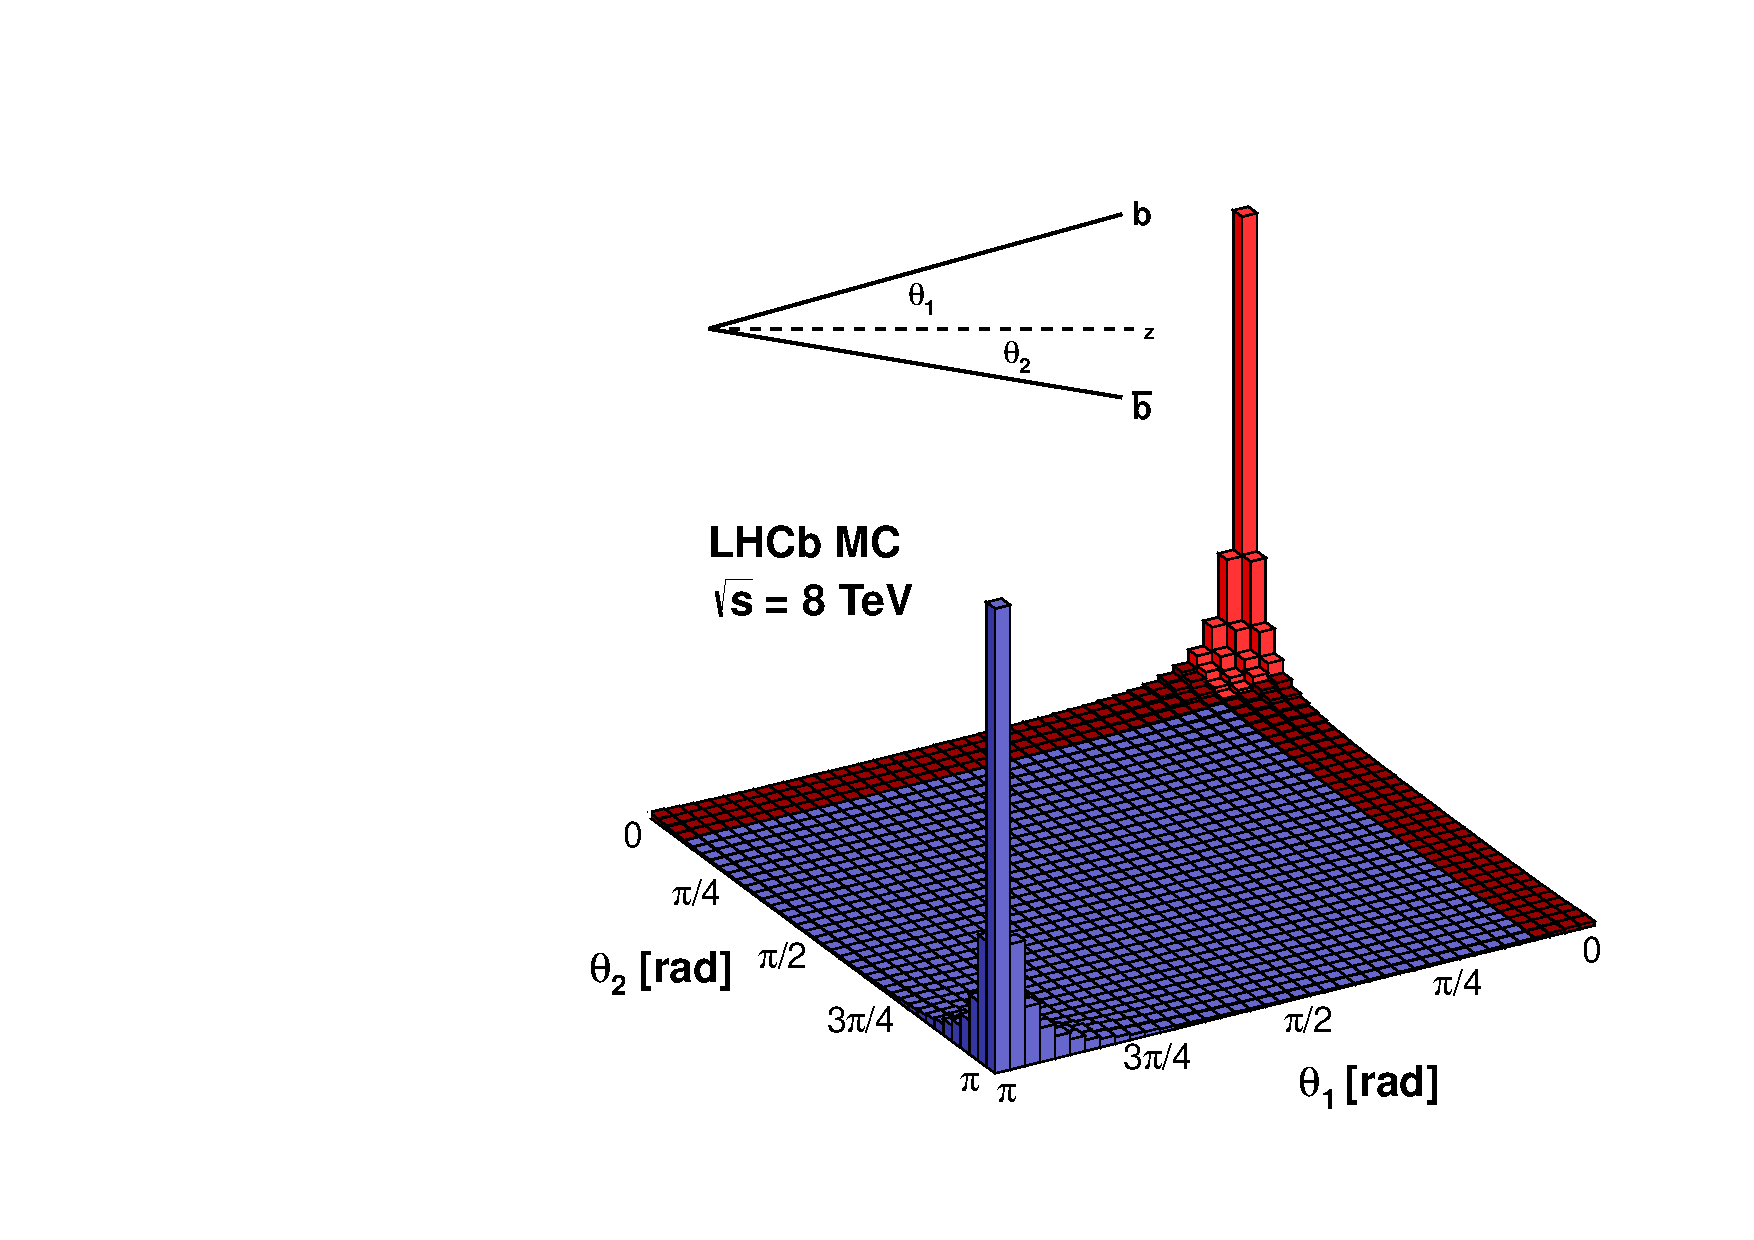
\includegraphics[width=0.5\textwidth]{fig/angle_plot.pdf}
	\caption{Winkelverteilung der $\bbbar$-Quark Paare zur Strahlachse bei einer Proton-Proton-Kollision. In rot ist der von \lhcb abgedeckte Winkelbereich dargestellt \cite{angle_plot}.}
	\label{fig:angle_plot} 
\end{figure} 
So liegen trotz der geringen Raumwinkelabdeckung etwa \SI{25}{\%} der $\bbbar$-Quark Paare innerhalb der Detektorakzeptanz. Weiterhin ist es bei $\lhcb$ wichtig, einzelne Prozesse möglichst detailliert aufzulösen. Dies ist umso einfacher, je weniger Proton-Proton-Kollisionen gleichzeitig stattfinden. Daher wird bei $\lhcb$ nicht die maximale vom $\lhc$ zur Verfügung gestellte Luminosität genutzt, sondern eine konstante Luminosität von etwa \SI[exponent-product = \cdot]{4e32}{cm^{-2}s^{-1}} \cite{LHC_statistik}. Diese wird eingestellt, indem der Überlapp der kollidierenden Protonenpakete bei $\lhcb$ kleiner ist als bei den anderen Experimenten. Da die Kollisionsrate mit aktuell \SI{20}{MHz} jedoch immer noch zu hoch ist, um alle Ereignisse direkt zu speichern, sind außerdem leistungsstarke Trigger vonnöten, die bereits eine erste Selektion der Daten vornehmen und möglichst viele Signalendzustände erhalten. Im Folgenden werden nun die einzelnen Komponenten des $\lhcb$-Detektors (Abbildung \ref{fig:det_plot}) in Anlehnung an \cite{Alves:2008zz}  erläutert.
\begin{figure}[htpb]
	\centering
		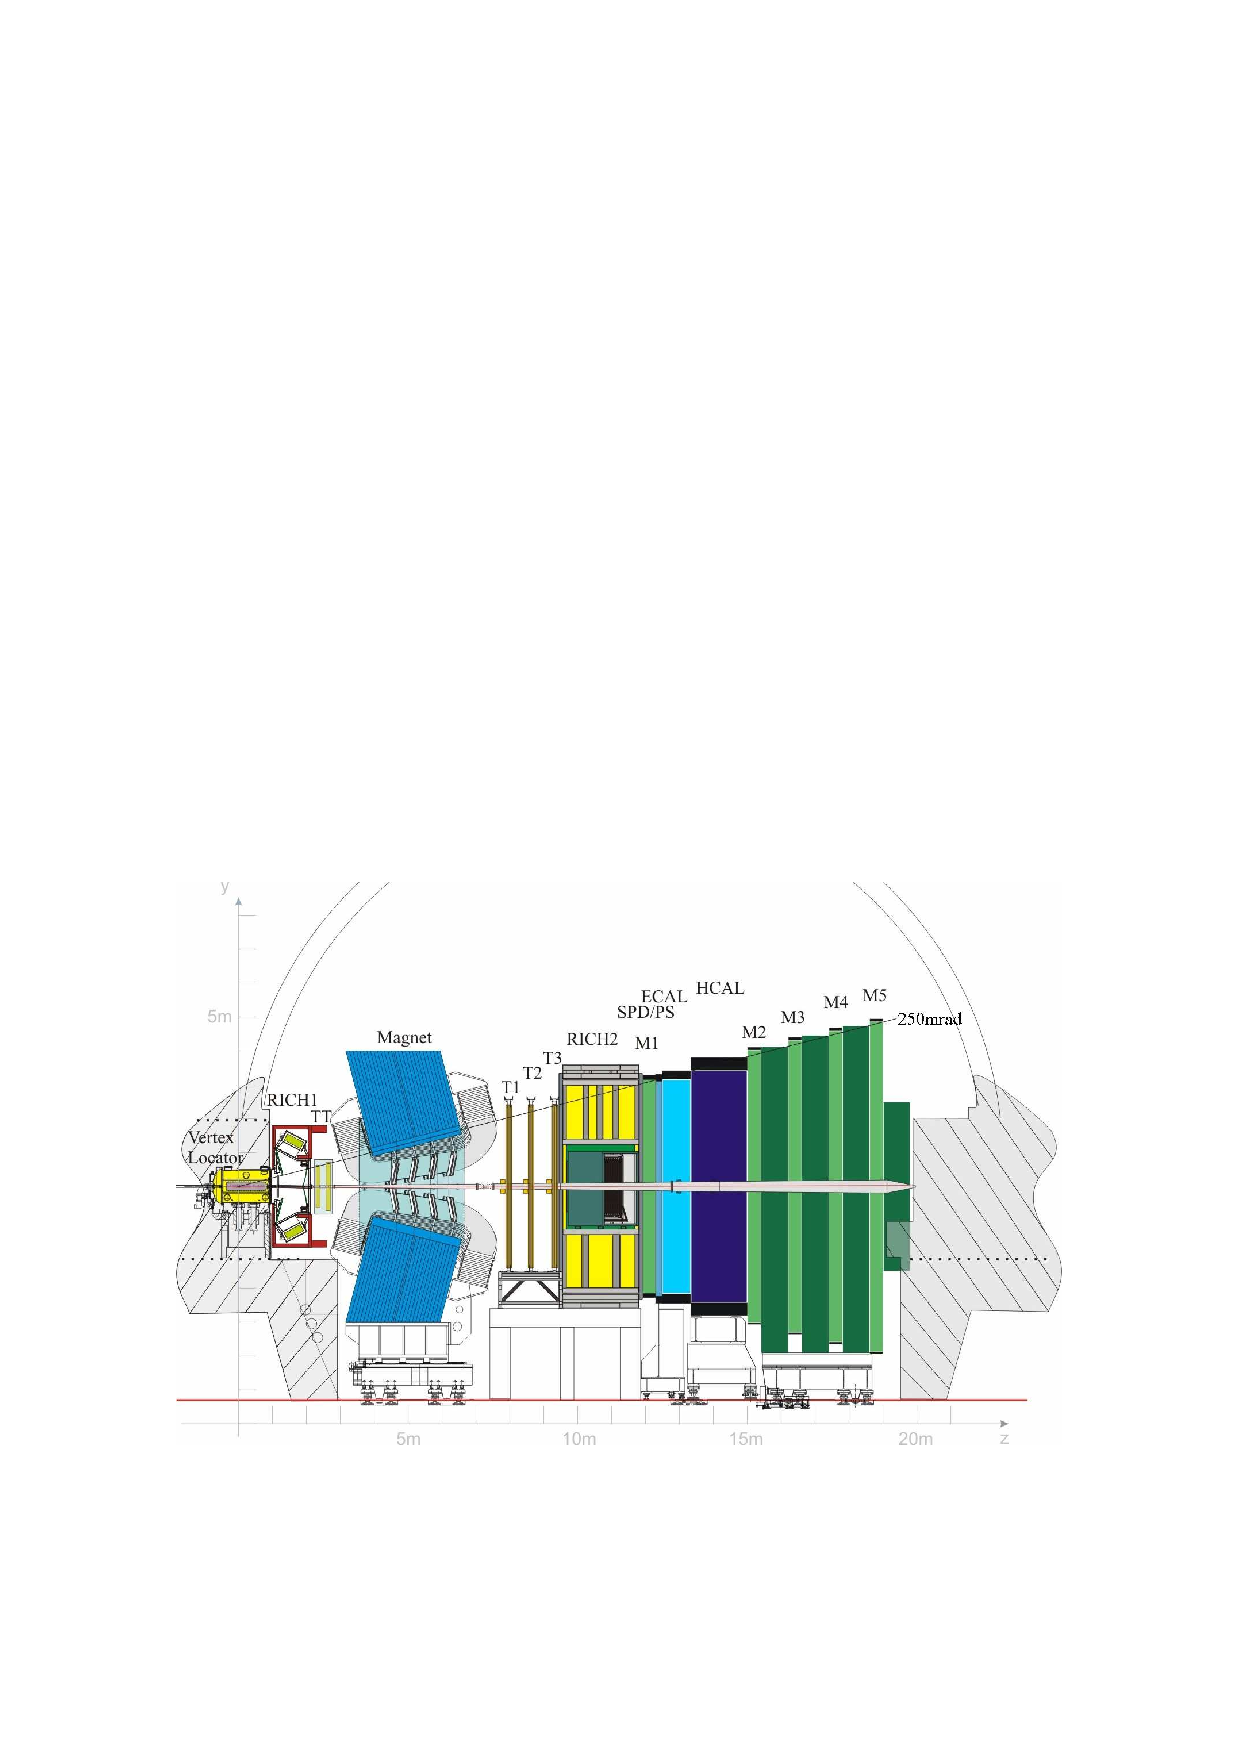
\includegraphics[width=0.8\textwidth]{fig/det_plot.pdf}
	\caption{Schematischer Aufbau des \lhcb-Detektors: Zu sehen sind der \velo, die beiden \rich-Detektoren, sowie das Tracking System mit Magnet, die Kalorimeter und die Myonenkammern. Der Kollisionspunkt wird links vom \velo umschlossen \cite{Alves:2008zz}.}
	\label{fig:det_plot} 
\end{figure} 

\subsection{Der Vertex-Locator}\label{sec:velo}

Der Vertex-Locator (\velo) ist die dem Kollisionspunkt nächste Detektorkomponente. Er gehört zum Tracking System und wird genutzt, um speziell Primär- und Sekundär-Vertices mit hoher Präzision aufzulösen. Der \velo ist aus einer Reihe von \num{21} halbkreisförmigen Silizium Modulen, die auf bis zu \SI{8}{mm} an den Strahl herangefahren werden können, aufgebaut. Diese messen jeweils die $r$ und $\phi$ Koordinaten des Treffers, den ein delektiertes Teilchen hinterlässt, und sind entlang der Strahlachse montiert (Abbildung \ref{fig:velo}).  
\begin{figure}[htpb]
	\centering
		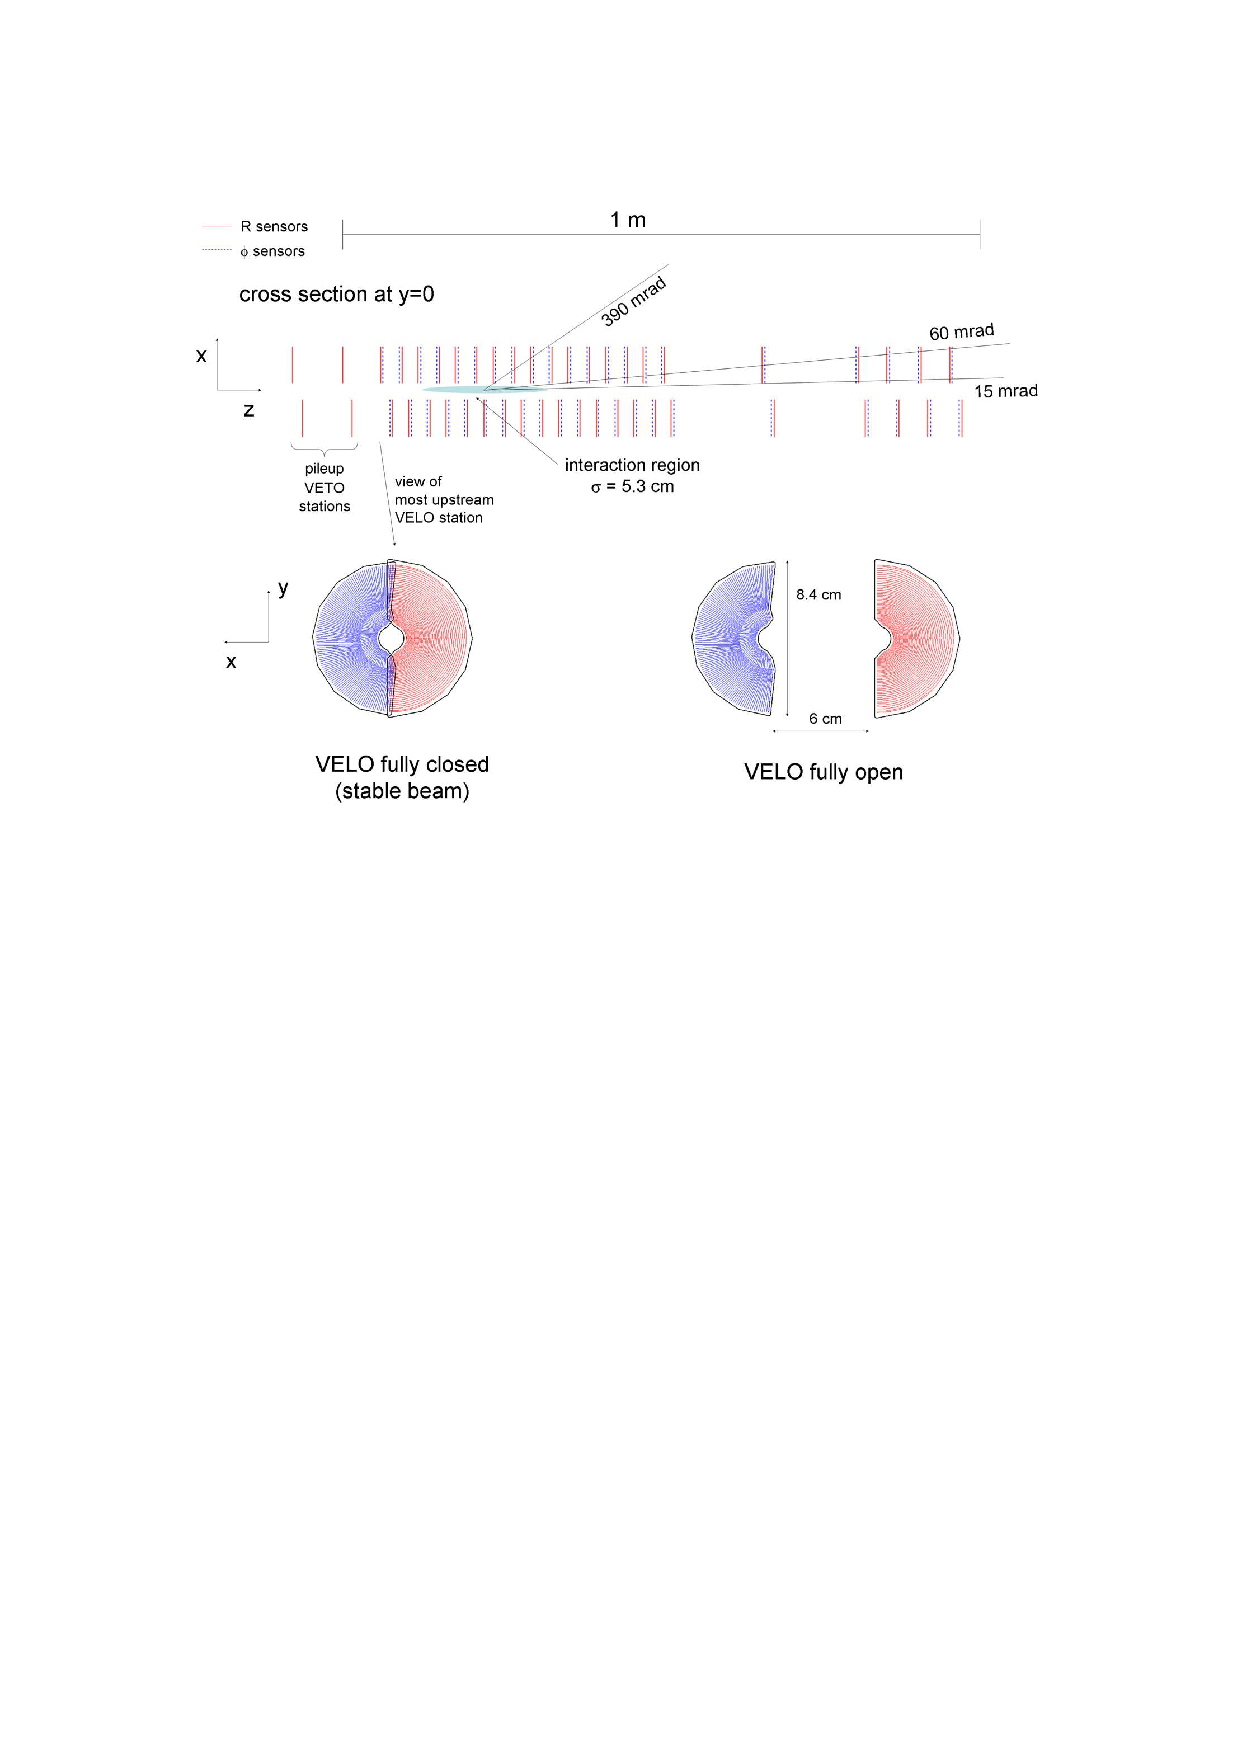
\includegraphics[width=0.7\textwidth]{fig/velo.pdf}
	\caption{Oben: Schnitt durch die $(x,z)$-Ebene des \velo bei $y=0$ bei geschlossenen Modulen. Unten: Sicht aus Strahlrichtung auf ein Modul im geschlossenen und geöffneten Zustand. Man erkennt die beiden Hälften zur $\phi$- (blau) und $r$-Messung (rot). \cite{Alves:2008zz}}
	\label{fig:velo} 
\end{figure} \\
Dabei wird zwischen einem inneren Teil nahe am Kollisionspunkt der Protonen und einem äußeren Teil strahlabwärts unterschieden. Bei einer Winkelakzeptanz von \SI{300}{mrad} bei \lhcb soll ein Teilchen mit diesem maximalen Winkel nun in mindestens drei Stationen Signale erzeugen, um rekonstruiert zu werden. Daraus folgt, dass der Abstand der inneren Stationen bei einem Radius der Sensoren von \SI{42}{mm} nicht größer als \SI{5}{cm} sein darf. Fordert man nun, unter der Annahme, dass einzelne Stationen nicht auslösen, dass in vier Stationen Signale erzeugt werden, kommt man auf einen Modulabstand von \SI{3{,}5}{cm} im inneren Teil des \velo. Außerdem wird durch diesen kleinen Abstand die mittlere Extrapolationsstrecke vom ersten gemessenen Treffer zum Vertex verkleinert.\\
Die untere Grenze der Winkelakzeptanz des \velo liegt bei \SI{15}{mrad} für Teilchen die, vom nominellen Interaktionspunkt der Protonen aus gesehen, bei $z=\SI{10{,}6}{cm}$ strahlabwärts entstehen.\\
Um die vollständige azimuthale Akzeptanz abzudecken, überlappen die beiden Detektorhälften jedes Moduls. Dies ist dadurch möglich, dass die $z$-Positionen der jeweiligen Hälften um \SI{1{,}5}{cm} zueinander verschoben sind (Abbildung \ref{fig:velo}).
 
\subsection{Die \rich-Detektoren}

Ein wichtiger Faktor bei \lhcb ist die Teilchenidentifikation, im Speziellen die Unterscheidung zwischen Pionen und Kaonen. Um diese gut zu realisieren, ist \lhcb mit zwei Ring-Imaging Cherenkov Detektoren, \richone und \richtwo, instrumentiert. Diese Detektoren nutzen den Cherenkov-Effekt, bei dem Teilchen sich in einem Medium mit einer höheren Geschwindigkeit bewegen als der Lichtgeschwindigkeit in diesem Medium. Diese Teilchen senden im Öffnungswinkel $\theta$ elektromagnetische Strahlung aus, wobei $\theta$ abhängig von der Geschwindigkeit der Teilchen ist:
\begin{equation}
\cos\left(\theta\right)=\frac{1}{n\beta}.
\end{equation}
Hier ist $n$ der Brechungsindex des durchflogenen Mediums und $\beta=$ \itshape\nicefrac{v}{c}\upshape. \\ 
Gemeinsam mit der Impulsinformation aus anderen Detektorkomponenten lässt sich dann gut zwischen verschiedenen Teilchen unterscheiden. Da sich das Impulsspektrum mit dem Polarwinkel (Winkel eines Teilchens zur Strahlachse) ändert, besteht das \rich-System aus den beiden Komponenten \richone und \richtwo. \richone identifiziert dabei Teilchen mit eher kleinen Impulsen von etwa \SI{1}{GeV\per c} bis \SI{60}{GeV\per c} \cite{Alves:2008zz} mit einer Mischung aus Aerogel und \cfourften, während \richtwo ein \cffour Gas verwendet und Teilchen mit größeren Impulsen im Bereich von $~$\SI{15}{GeV\per c} bis \SI{100}{GeV\per c} \cite{Alves:2008zz} unterscheidet. Wegen dieser unterschiedlicher Impulsbereichen ist \richone unmittelbar hinter dem \velo positioniert, während \richtwo erst hinter dem weiteren Tracking-System mit Magnet positioniert ist (Abbildung \ref{fig:det_plot}). 

\subsection{Das Tracking-System}


Das Tracking-System teilt sich in den Tracker Turicensis (\ttracker) und die drei Tracking-Stationen T$1$ bis T$3$ . Bei den Tracking-Stationen T$1$ bis T$3$ unterscheidet man weiter einen inneren Bereich nahe der Strahlröhre, den Inner Tracker (\intr), und entferntere Bereiche von der Strahlröhre, den Outer Tracker (\ot). Technologisch sind sowohl der \ttracker als auch der \intr Silizium Tracker (\st). Zum Tracking-System gehört außerdem ein Dipolmagnet mit einer integrierten Magnetfeldstärke von \SI{4}{Tm}, der zwischen dem \ttracker und dem restlichen Trackingsystem positioniert ist, sowie der in Abschnitt \ref{sec:velo} beschriebene \velo.\\
Die \st sind Detektoren aus Siliziumstreifen. Bei einer Breite der Siliziumstreifen von \SI{200}{\micro m} im \intr und \ttracker wird eine räumliche Auflösung von \SI{50}{\micro m} erreicht. Der \ttracker ist unmittelbar hinter dem \richone und vor dem Magneten installiert. Er ist \SI{150}{cm} breit und hat eine Höhe von \SI{130}{cm}. Der \intr ist in den drei Stationen  T$1$ bis T$3$ hinter dem Magneten im zentralen Bereich um das Strahlrohr installiert. Er deckt eine Fläche von \SI{120}{cm} Breite und \SI{40}{cm} Höhe ab (Abbildung \ref{fig:it}). 
\begin{figure}[htpb]
	\centering
		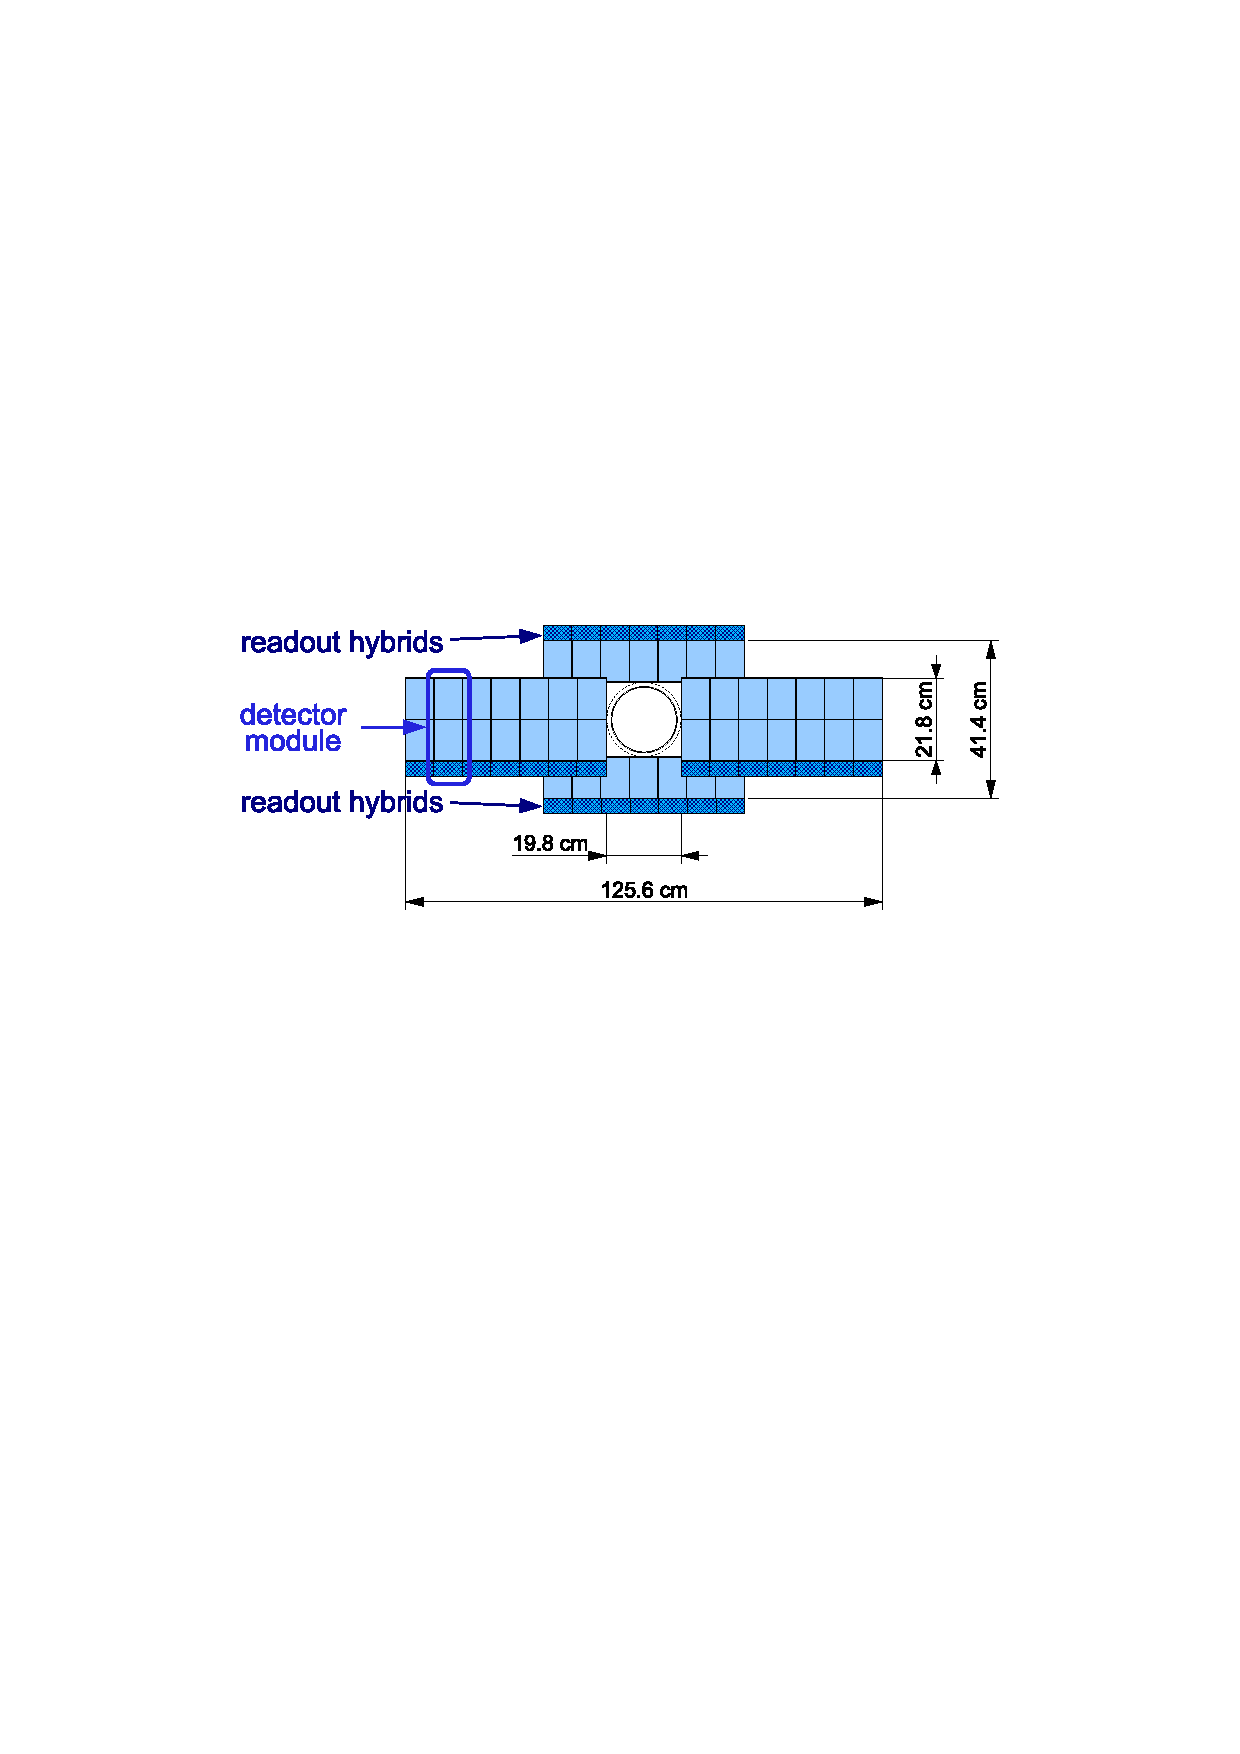
\includegraphics[width=0.7\textwidth]{fig/IT.pdf}
	\caption{Schematische Ansicht einer Schicht des \intr mit Auslesektronik. Eine Station setzt sich aus vier solcher Schichten zusammen, wobei die mittleren Schichten gegen die $(x,y)$-Ebene gekippt sind, um zusätzliche Winkelinformationen zu gewinnen. \cite{Alves:2008zz}}
	\label{fig:it} 
\end{figure}\\
Bei dem \ot handelt es sich um einen Detektor aus gasgefüllten Driftröhrchen. Dabei wird in den Driftröhrchen die Driftzeit ionisierter Gasatome und ihrer Elektronen gemessen und aus dieser Driftzeit auf die Ionisationsstelle geschlossen. Das Gasgemisch in den Driftröhrchen setzt sich dabei zu \SI{70}{\%} aus Argon, zu \SI{28{,}5}{\%} aus \cotwo  und zu \SI{1{,}5}{\%} aus {\ensuremath{\rm O_2}\xspace}  zusammen. Durch diese Zusammensetzung garantiert es möglichst schnelle Driftzeiten von unter \SI{50}{ns} und trotz allem eine hohe räumliche Auflösung von \SI{200}{\micro m}. Die Impulsauflösung des \ot beträgt $\frac{\delta p}{p}\approx\SI{0{,}4}{\%}$, bei einer Gesamtrekonstruktionseffizienz von \SI{80}{\%} \cite{Alves:2008zz}.\\
Alle Trackingstationen, das heißt sowohl der \ttracker als auch die Stationen T$1$ bis T$3$, sind aus jeweils vier Lagen aufgebaut, wobei die mittleren Lagen jeweils um $\pm$\SI{5}{\degree} um die Strahl-Achse gedreht sind, sodass sich die $y$-Koordinate eines Treffers, den ein Teilchen hinterlässt, bestimmen lässt. 

\subsection{Kalorimeter}

Die Kalorimeter haben verschiedene Aufgaben zu erfüllen. Zum einen unterstützen sie die \en-, \g- und Hadronenidentifizierungen, zum anderen messen sie Teilchenenergien und Positionen. Weiterhin selektieren sie Kandidaten für die erste Triggerstufe, den L$0$-Trigger, der bereits \SI{4}{\micro s} nach einer Wechselwirkung erste Entscheidungen trifft. Insgesamt folgt der Kalorimeteraufbau bei \lhcb der klassischen Abfolge. Auf ein elektromagnetisches Kalorimeter (\ecal) folgt ein hadronisches Kalorimeter (\hcal). Das \ecal ist dabei für die \en-Identifikationen verantwortlich.\\
Um  Untergründe von geladenen Pionen zu unterdrücken, ist vor dem \ecal der Preshower (\presh) installiert . Für die Trigger werden Untergründe von \piz mit hoher Transversalenergie $\et$ durch den Scintillating Pad Detector (\spd) unterdrückt.
Da die Trefferdichte über die Kalorimeterfläche um zwei Größenordnung variiert, ist die laterale Aufteilung der Kalorimeter je nach Abstand zur Strahlröhre unterschiedlich und wird mit der Entfernung zur Strahlröhre größer (Abbildung \ref{fig:kalos}).
\begin{figure}[htpb]
	\centering
		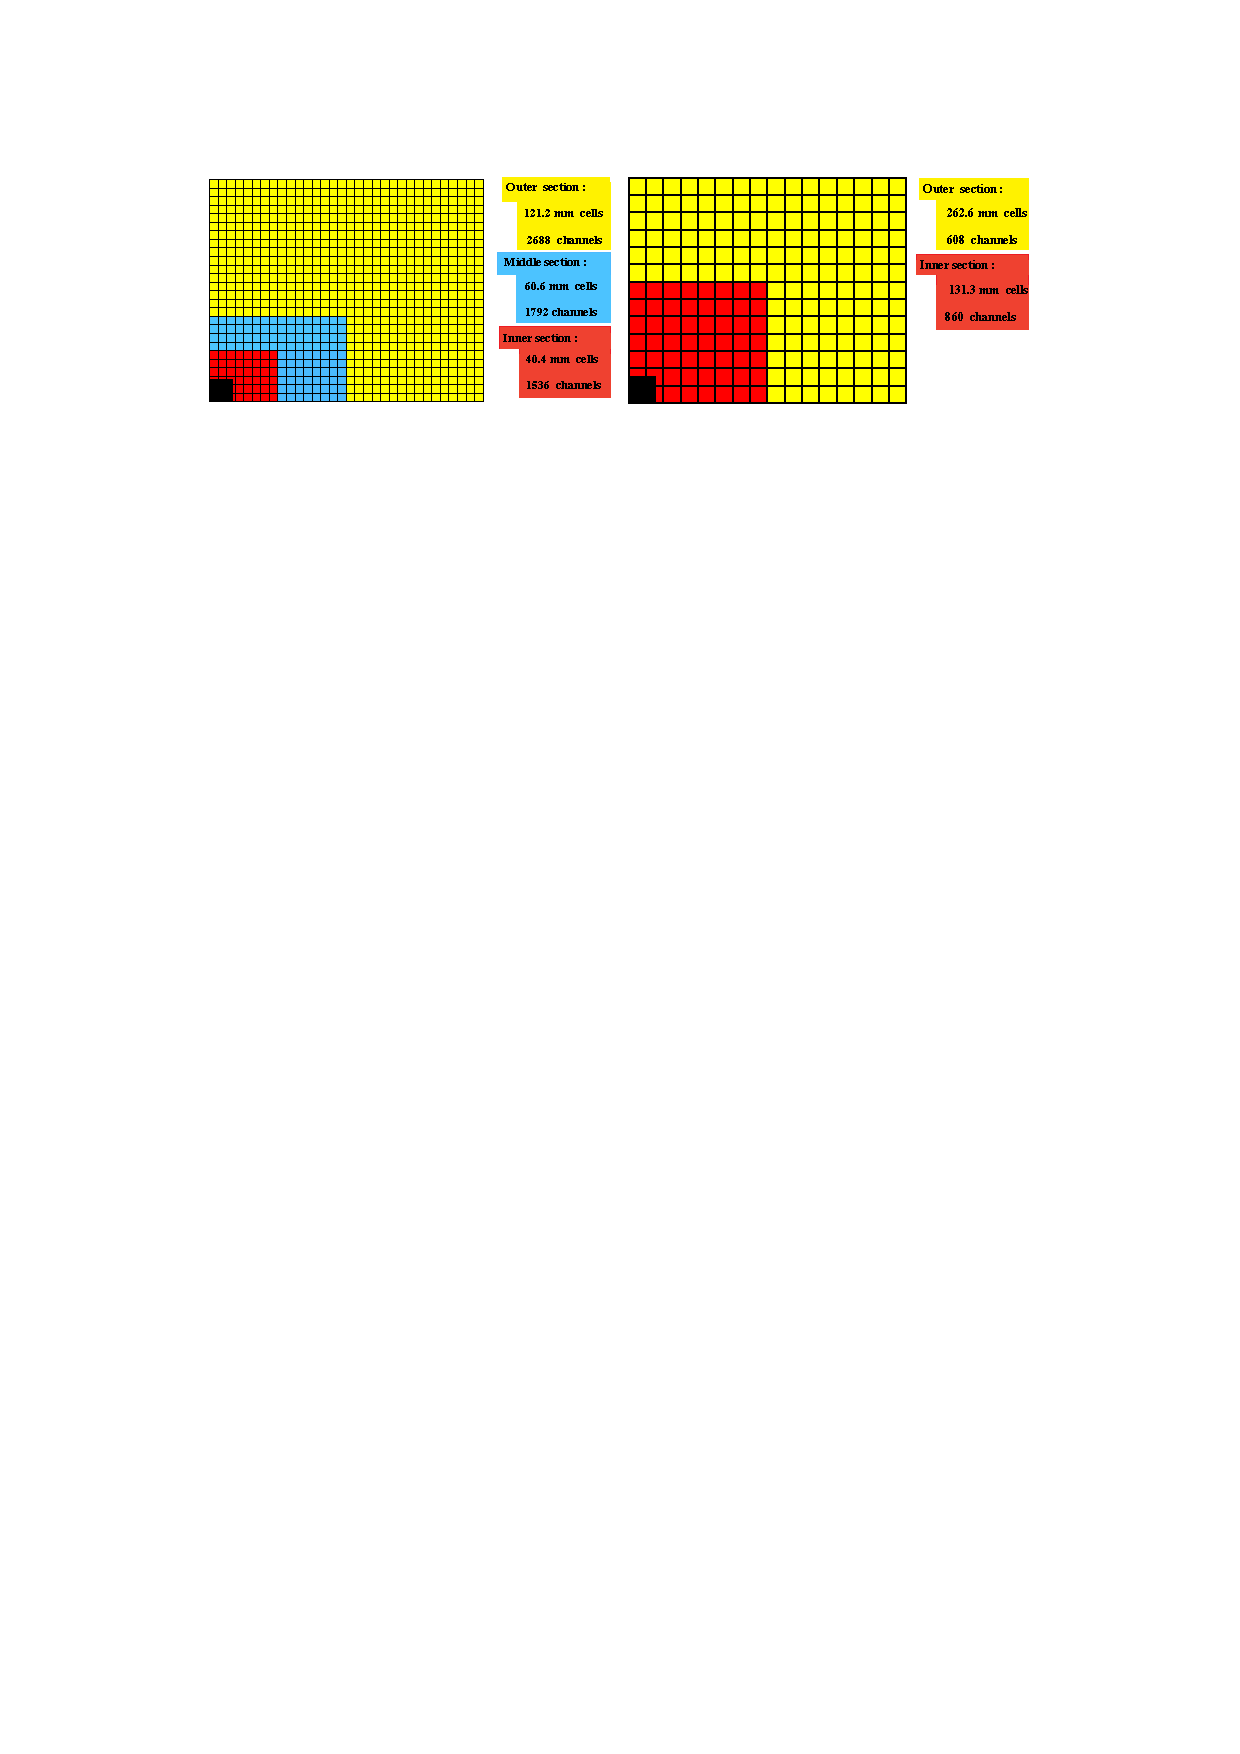
\includegraphics[width=0.9\textwidth]{fig/kalos.pdf}
	\caption{Laterale Aufteilung von \presh, \spd und \ecal (links) sowie vom \hcal (rechts). Zu sehen ist ein Viertel der Vorderansicht des Detektors. In schwarz ist der für das Strahlrohr ausgesparte Bereich dargestellt. \cite{Alves:2008zz}}
	\label{fig:kalos} 
\end{figure}

\subsection{Die Myonenkammern}

Die Detektion von Myonen ist von fundamentaler Wichtigkeit für \lhcb. Sowohl in vielen \CP-sensitiven Zerfällen, wie $\Bd\rightarrow\jpsi\KS$, in dem das \jpsi im Zerfall nach zwei Myonen rekonstruiert wird, als auch in seltenen $\B$-Zerfällen mit flavour-ändernden neutralen Strömen, wie $\Bs\rightarrow\mup\mun$, sind sie in Endzuständen zu finden. Bei \lhcb gibt es fünf Myonenkammern. Die Kammer M$1$ befindet sich vor den Kalorimetern, während M$2$ bis M$5$ hinter diesen positioniert sind. Die einzelnen Stationen sind dabei von \SI{80}{cm} dicken Eisenabsorbern durchzogen, sodass der Minimalimpuls eines Myons, um alle fünf Stationen zu passieren, \SI{6}{GeV} betragen muss. Die Stationen M$1$ bis M$3$ haben eine relativ hohe räumliche Auflösung entlang der $x$-Koordinate. Sie werden vor allem genutzt, um die Spurrichtungen zu identifizieren und den Transversalimpuls \pt der Myonkandidaten mit einer Auflösung von \SI{20}{\%} zu messen. Die Stationen M$4$ und M$5$ dienen dagegen eher der Teilchenidentifikation eindringender Myonen.  

\subsection{Trigger}\label{sec:trigger}

Das \lhcb-Experiment arbeitet nicht, wie die Vielzweckexperimente \atlas und \cms, bei der maximalen vom \lhc zur Verfügung gestellten Luminosität von $L\approx\SI[exponent-product = \cdot]{7e33}{cm^{-2}s^{-1}}$, sondern bei einer Luminosität von $L=\SI[exponent-product = \cdot]{4e32}{cm^{-2}s^{-1}}$, um im Idealfall pro Protonenpaketkollision exakt eine Proton-Proton-Wechselwirkung aufzunehmen. Trotzdem muss die Datenrate von etwa \SI{20}{MHz} noch auf etwa \SI{4}{kHz} reduziert werden, um gespeichert werden zu können. Dazu stehen zwei Trigger-Stufen zur Verfügung: Die erste Stufe (L$0$) arbeitet synchron zur Wechselwirkungsrate von \SI{40}{MHz} und reduziert diese auf \SI{1}{MHz}, woraufhin die zweite Trigger-Stufe, der High-Level-Trigger (HLT) unabhängig von der Wechselwirkungsrate die Daten weiterverarbeitet. Bei einer Luminosität von $L=\SI[exponent-product = \cdot]{4e32}{cm^{-2}s^{-1}}$ werden Ereignisse, die ein \B-Meson beinhalten, mit einer Rate von etwa \SI{15}{kHz} erzeugt. Weiterhin sind viele partielle Zerfallsbreiten der \B-Mesonen kleiner als $10^{-3}$, sodass das  Triggersystem dahingehend optimiert ist, diese interessanten Zerfälle für nachfolgende Analysen mit maximaler Effizienz zu selektieren, während die in der hadronischen Umgebung entstehenden Untergründe maximal unterdrückt werden \cite{Alves:2008zz}.\\
Bei dem Level-0-Trigger handelt es sich um einen reinen Hardware-Trigger. Er versucht zunächst die Hadronen, Elektronen und Photonen mit maximalen Transversalenergien \et, sowie die beiden Myonen mit den höchsten Transversalimpulsen \pt zu identifizieren. Dazu besteht der L$0$ aus drei Komponenten: Einem L$0$-pile-up-System, dem L$0$-Kalorimeter-Trigger und dem L$0$-Myon-Trigger. Ziel des pile-up-Systems ist dabei die Unterscheidung zwischen Events mit einer oder mehreren sichtbaren Proton-Proton-Wechselwirkungen. Die Kalorimeter- und Myon-Komponenten suchen für die entsprechenden Teilchen nach den maximalen \et beziehungsweise \pt.\\
Der HLT ist eine C++ Anwendung und läuft auf der sogenannten Event Filter Farm (EFF), einem Großrechner am \cern. Jede Anwendung hat dabei vollen Zugriff auf alle Informationen eines Events. Prinzipiell könnten hier also bereits Selektionsschritte durchgeführt werden. Da die Datenrate, die vom L$0$-Trigger kommt, jedoch sehr groß ist, besteht der HLT aus zwei Stufen. Der HLT$1$ rekonstruiert dabei die Teilchenkandidaten, die der L$0$ übergibt, im \velo und in den Tracking-Stationen. Außerdem werden hier für Photonen und neutrale Pionen die Abwesenheit geladener Teilchen bestätigt, die mit diesen beiden ungeladenen Kandidaten assoziiert werden könnten. Insgesamt hat der HLT$1$ die Aufgabe, die Datenrate so weit zu reduzieren, dass im nächsten Schritt, dem HLT$2$, eine vollständige Mustererkennung möglich ist. Bei einer ausreichend niedrigen Datenrate rekonstruiert der HLT$2$ dann schon teilweise spezifische \B-Zerfälle.

\subsection{\lhcb Software}

Die \lhcb-Software basiert auf dem \gaudi-Framework \cite{gaudi}, in dem verschiedene Software Pakete ausgeführt werden. Die Reihenfolge, in der die verschiedenen Pakete ausgeführt werden, ist in Abbildung \ref{fig:software} dargestellt.
\begin{figure}[htpb]
	\centering
		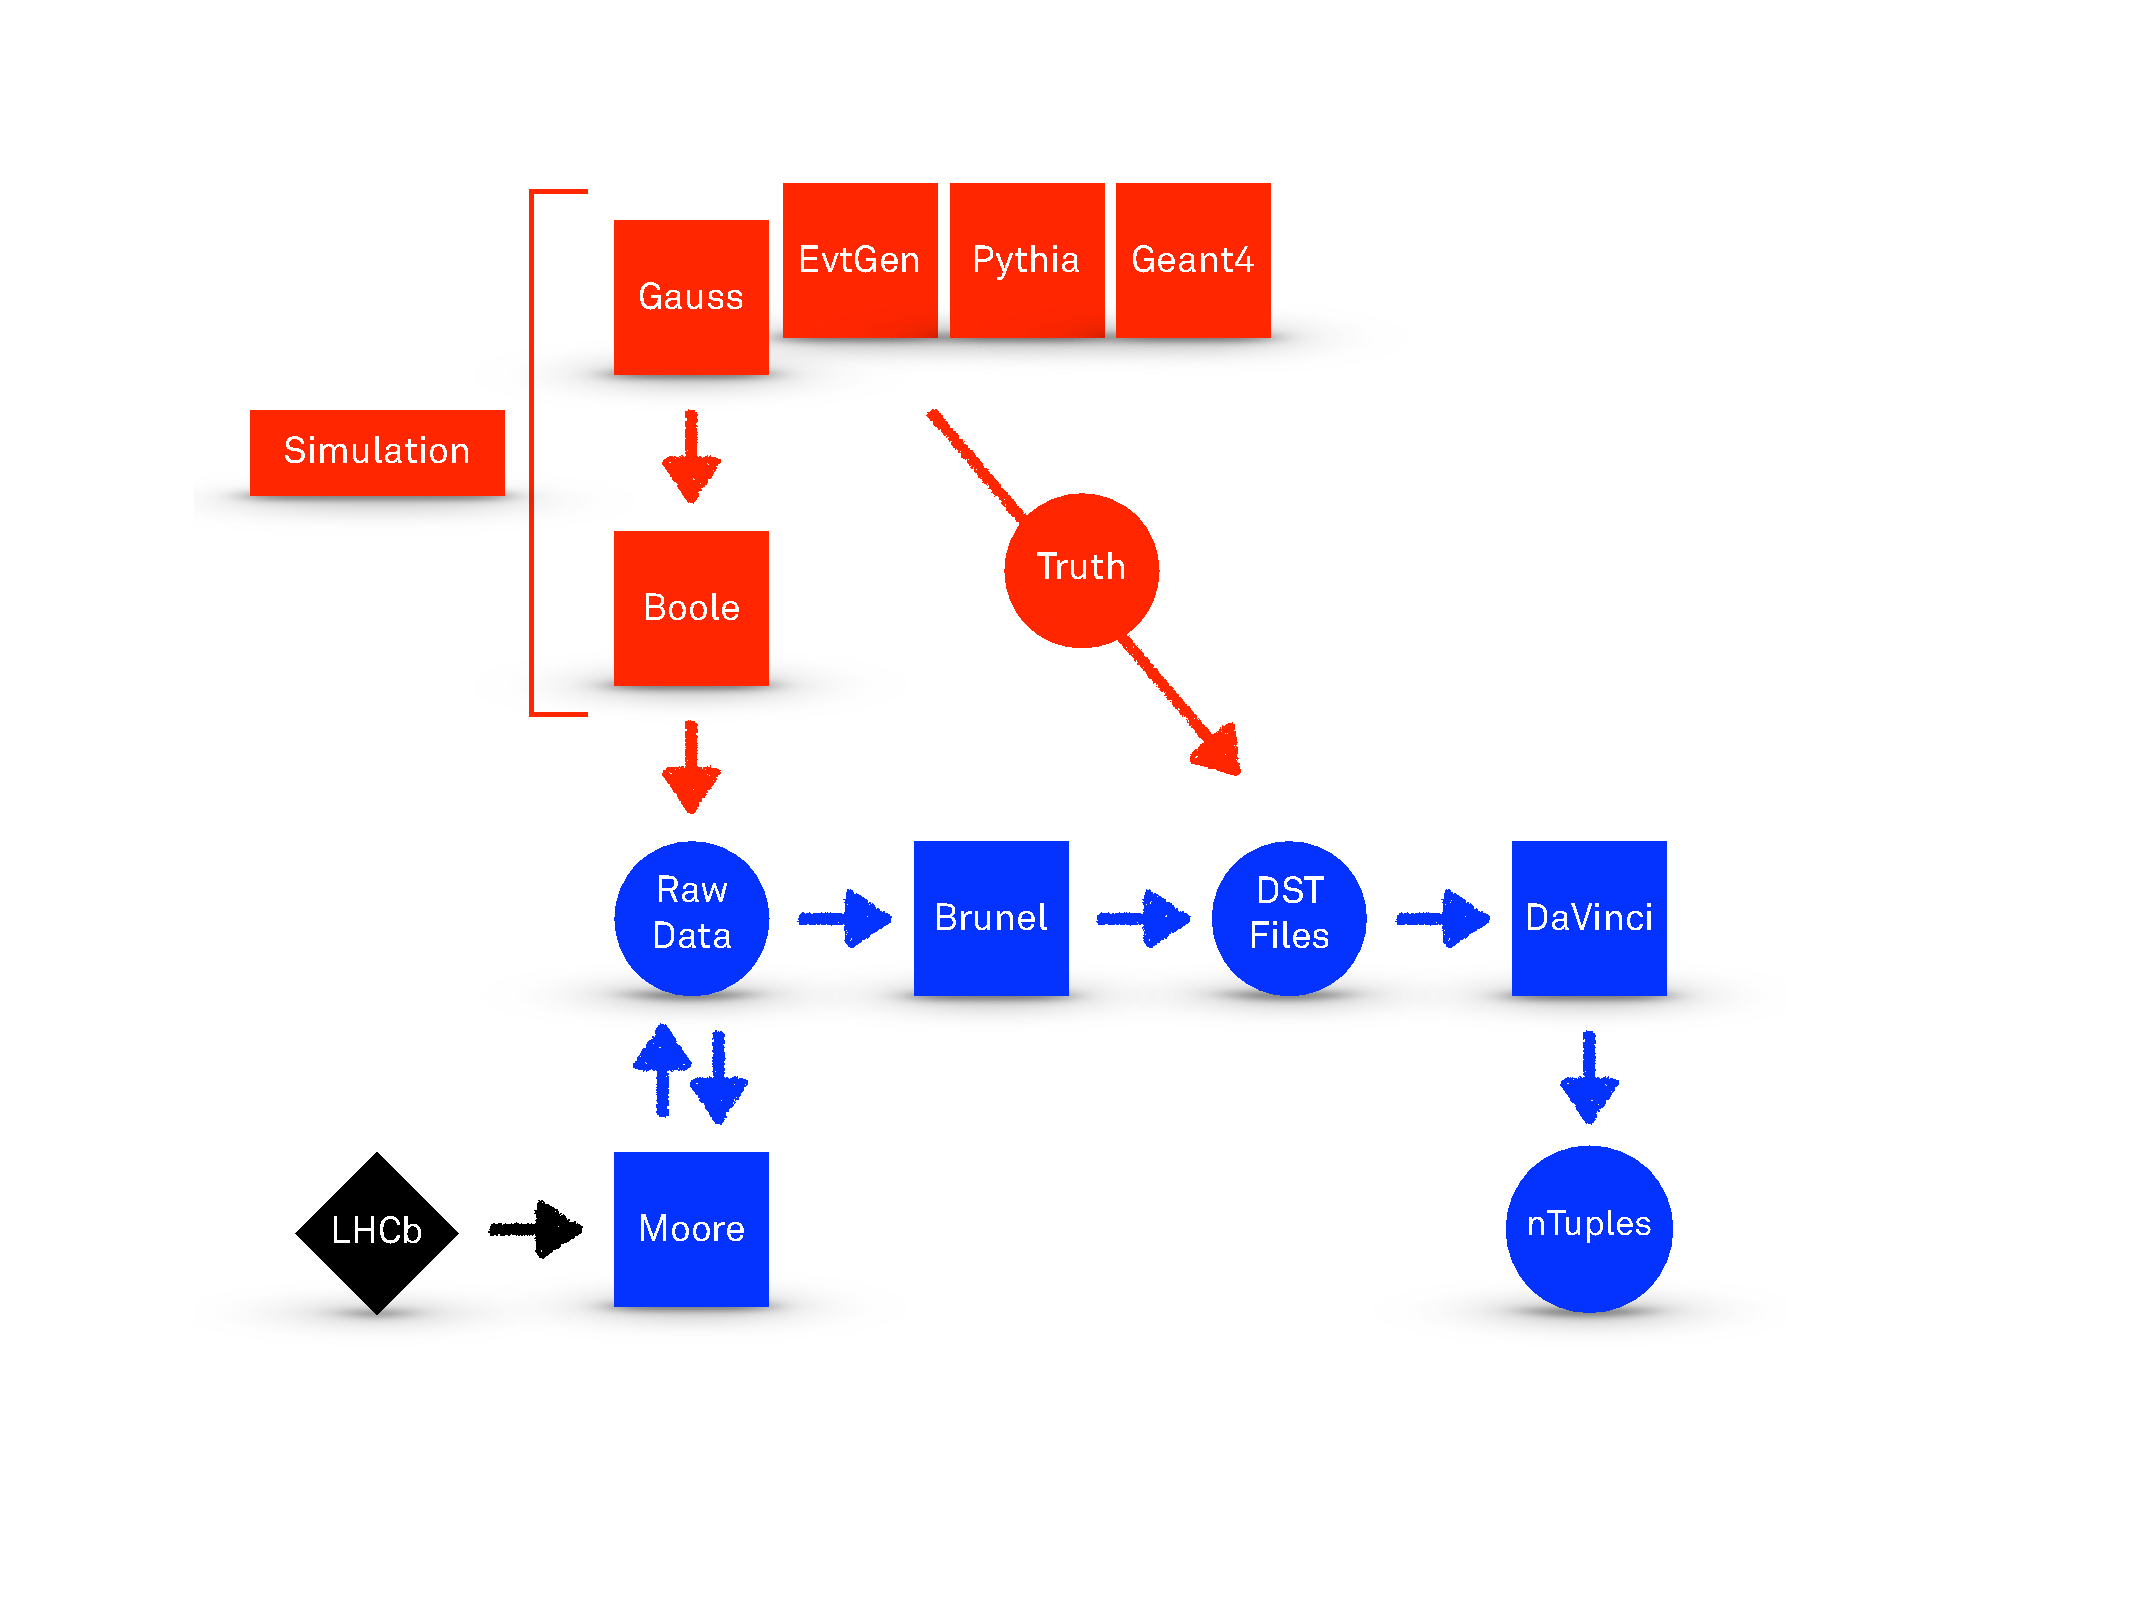
\includegraphics[width=0.7\textwidth]{fig/software.pdf}
	\caption{Abfolge der Datenprozessierung innerhalb der \lhcb-Software. In rot die Schritte zu Simulation von Daten, in blau die Prozessierung realer Daten. Die Software-Pakete sind dabei in Rechtecken, die übergebenen Datenformate in Kreisen dargestellt.}
	\label{fig:software} 
\end{figure}
Der erste Eingriff in die vom Detektor aufgenommen Daten passiert, wie in Abschnitt \ref{sec:trigger} beschrieben, beim HLT durch das Software Paket \moore \cite{moore}. Danach werden die Rohdaten in \brunel \cite{brunel} rekonstruiert und die Teilchen in sogenannten Protoparticles zusammengefasst. Diese Protoparticles haben dann sowohl Spurinformationen über das betreffende Teilchen, als auch Teilchenidentifikationsinformationen (PID-Informationen). Die nun als Data Summary Tape Dateien (DST's) vorliegenden Daten werden anschließen in \davinci \cite{davinci} weiter für die Analysen aufbereitet. Hier läuft sowohl eine erste Vorselektion, das sogenannte Stripping, in der die einzelnen Analysen speziell für ihre Bedürfnisse Schnitte auf physikalische Observablen definieren, als auch die finale Rekonstruktion der unterschiedlichen Prozesse. Ebenso wird an dieser Stelle das Flavour Tagging durchgeführt. Nachdem die Daten nun in Form von sogenannten nTuplen vorliegen, können diese mit \root \cite{root}, einer Sammlung von C++ Bibliotheken, die auf statistische Analysen der Hochenergiephysik spezialisiert sind, analysiert werden. Besonders hervorzuheben ist hier die \roofit \cite{roofit} Bibliothek, die bereits viele Parametrisierungen zur statistischen Modellierung der Daten beinhaltet. \\
Die Simulation von Daten wird bei \lhcb im \gauss Paket \cite{gauss} umgesetzt. Dieses ruft zunächst die Programmpakete \evtgen \cite{evtgen}, \pythia \cite{pythia6,pythia8}, das mit einer speziellen \lhcb Konfiguration \cite{lhcbconf} läuft, und \geant \cite{geant1,geant2} auf, die nacheinander die Proton-Proton-Kollisionen, den Hadronisationsprozess und die Wechselwirkung mit dem Detektor simulieren. Anschließend folgt \boole \cite{boole}, das die Daten digitalisiert, sodass diese anschließend wie die rohen Detektordaten verwendet werden können. Die Wahrheits- (Truth-)Informationen werden ebenfalls gespeichert und sind am Ende der Prozessierung bei der Analyse abrufbar. So sind in den Simulationen, neben den Detektorantworten, auch die anfangs generierten Zustände bekannt.  
